\section{Alex Pitcher Report - Part II}


\begin{marginfigure}
\checkoddpage \ifoddpage \forcerectofloat \else \forceversofloat \fi
\centering
 \frame{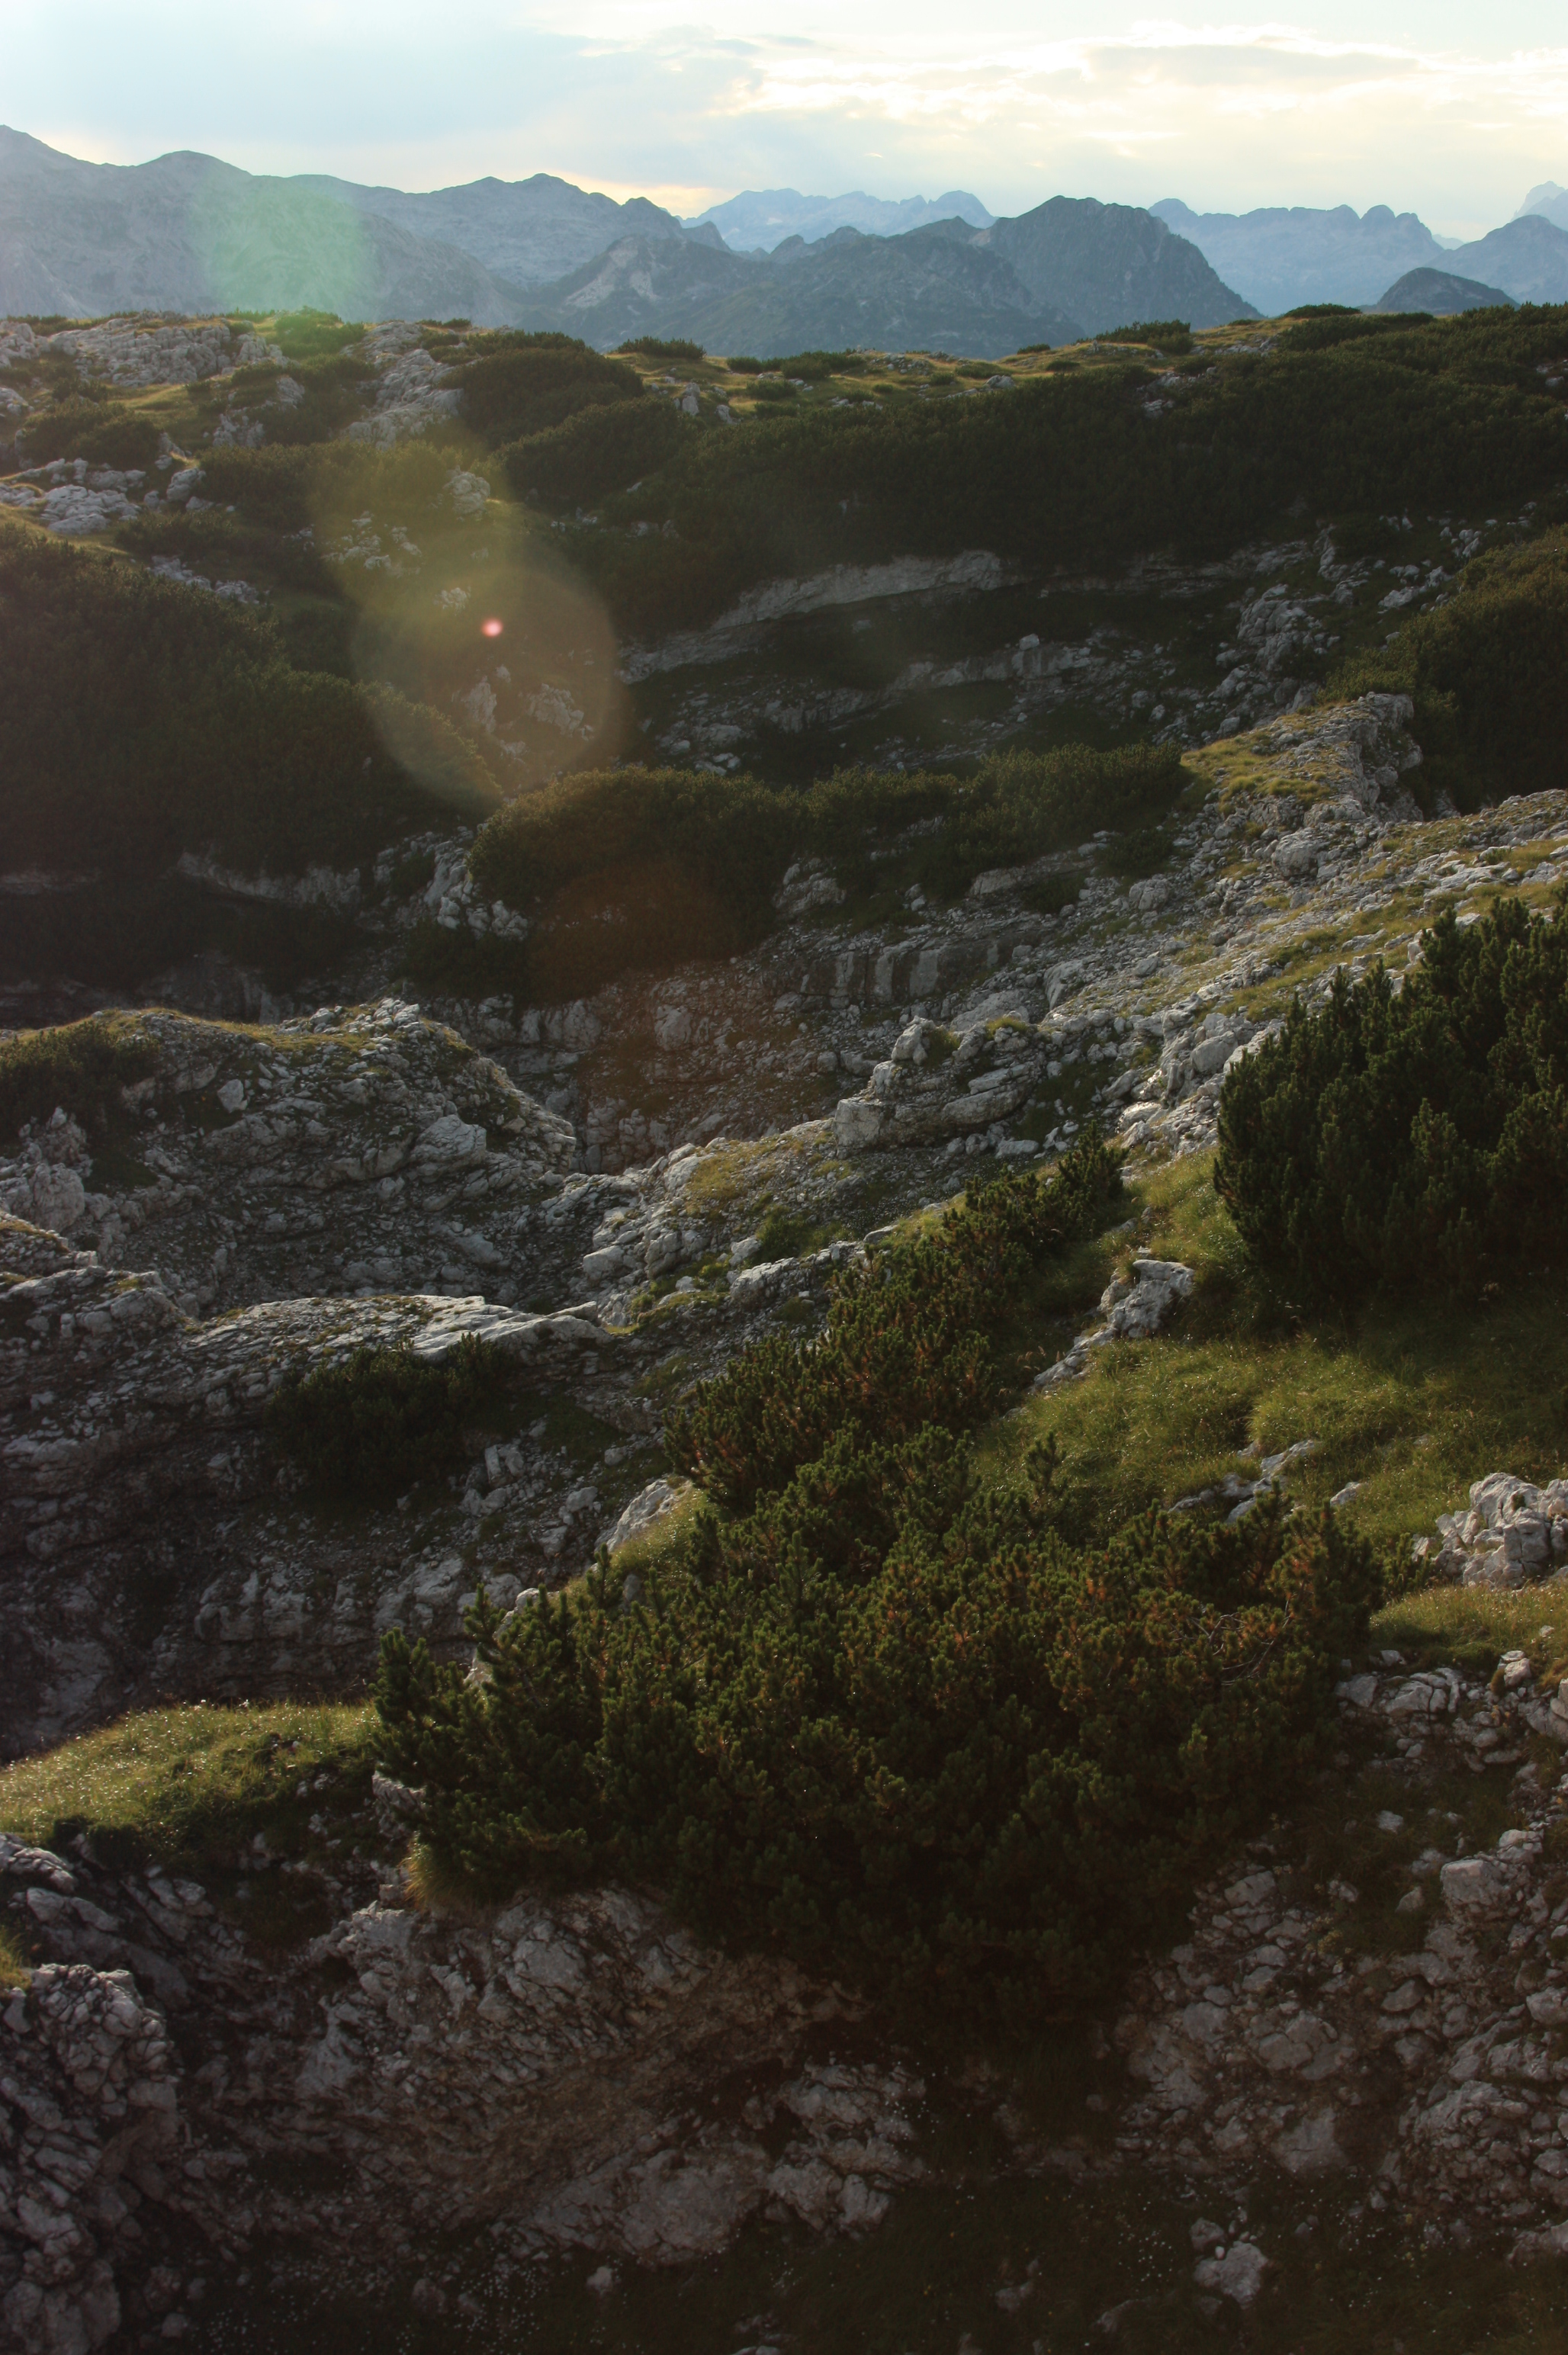
\includegraphics[width=\linewidth]{2011/alex_pitcher_award/2011-08-01-18.16.41-Gergely Ambrus-Canon450D-IMG_0803-Plateau--orig.jpg}} 
 \caption{The plateau. \pic{Gergely Ambrus}}
 \label{plateau}
\end{marginfigure}




\subsection{Second trip to underground camp}

Even more determined to get underground now, I rather lazily set to work
patching my suit together. On my previous excursion through the
\passage{Pink} series I had ripped it badly. It was now almost entirely
missing a backside/ back, one of the arms had a rip as long as my
forearm along it and the knees had large holes in them that threatened
to widen. As we spent a sunny afternoon in the \passage{Bivi} catching up, the
covering of my suit began more and more to resemble patchwork yet it
also meant I was almost ready to return to underground camp.

Unfortunately, the next day came and went as Dave still didn't feel
entirely certain about his own physical state. Then, late in the
afternoon of the following day, we finally headed down to camp. The trip
down was over much more quickly than my previous journey to underground
camp. Our `mission' for this pushing trip was to investigate a hole in
the side of \passage{Big Rock Candy Mountain} that Dave had noticed the
previous year. After a night's rest, we set off to do just that.

\margininbox{Big Rock traverse}{
     \begin{itemize}
    \item Jonathon Hardman
    \item Dave Wilson
    \end{itemize}}{\explo}

We lugged a drill and some rope to the other end of \passage{Friendship
Gallery} (the drill, to hopefully make rigging down this monster pitch
an easier task). The plan was to rig a traverse across the mud slope that
formed the beginning of the pitch to the other side then drop down from
there. Hopefully, this would have then provided access to the hole much
easier. In hindsight, it would have been best to have a look down the
pitch first and ensure that we were going about this mission the best
way possible but due to the size and the precarious nature of the pitch
itself, we both seemed reluctant to do so.




    \begin{figure*}[t!]
        \checkoddpage \ifoddpage \forcerectofloat \else \forceversofloat \fi
        \centering
        \begin{subfigure}[t]{0.68\textwidth}
            \centering
            \frame{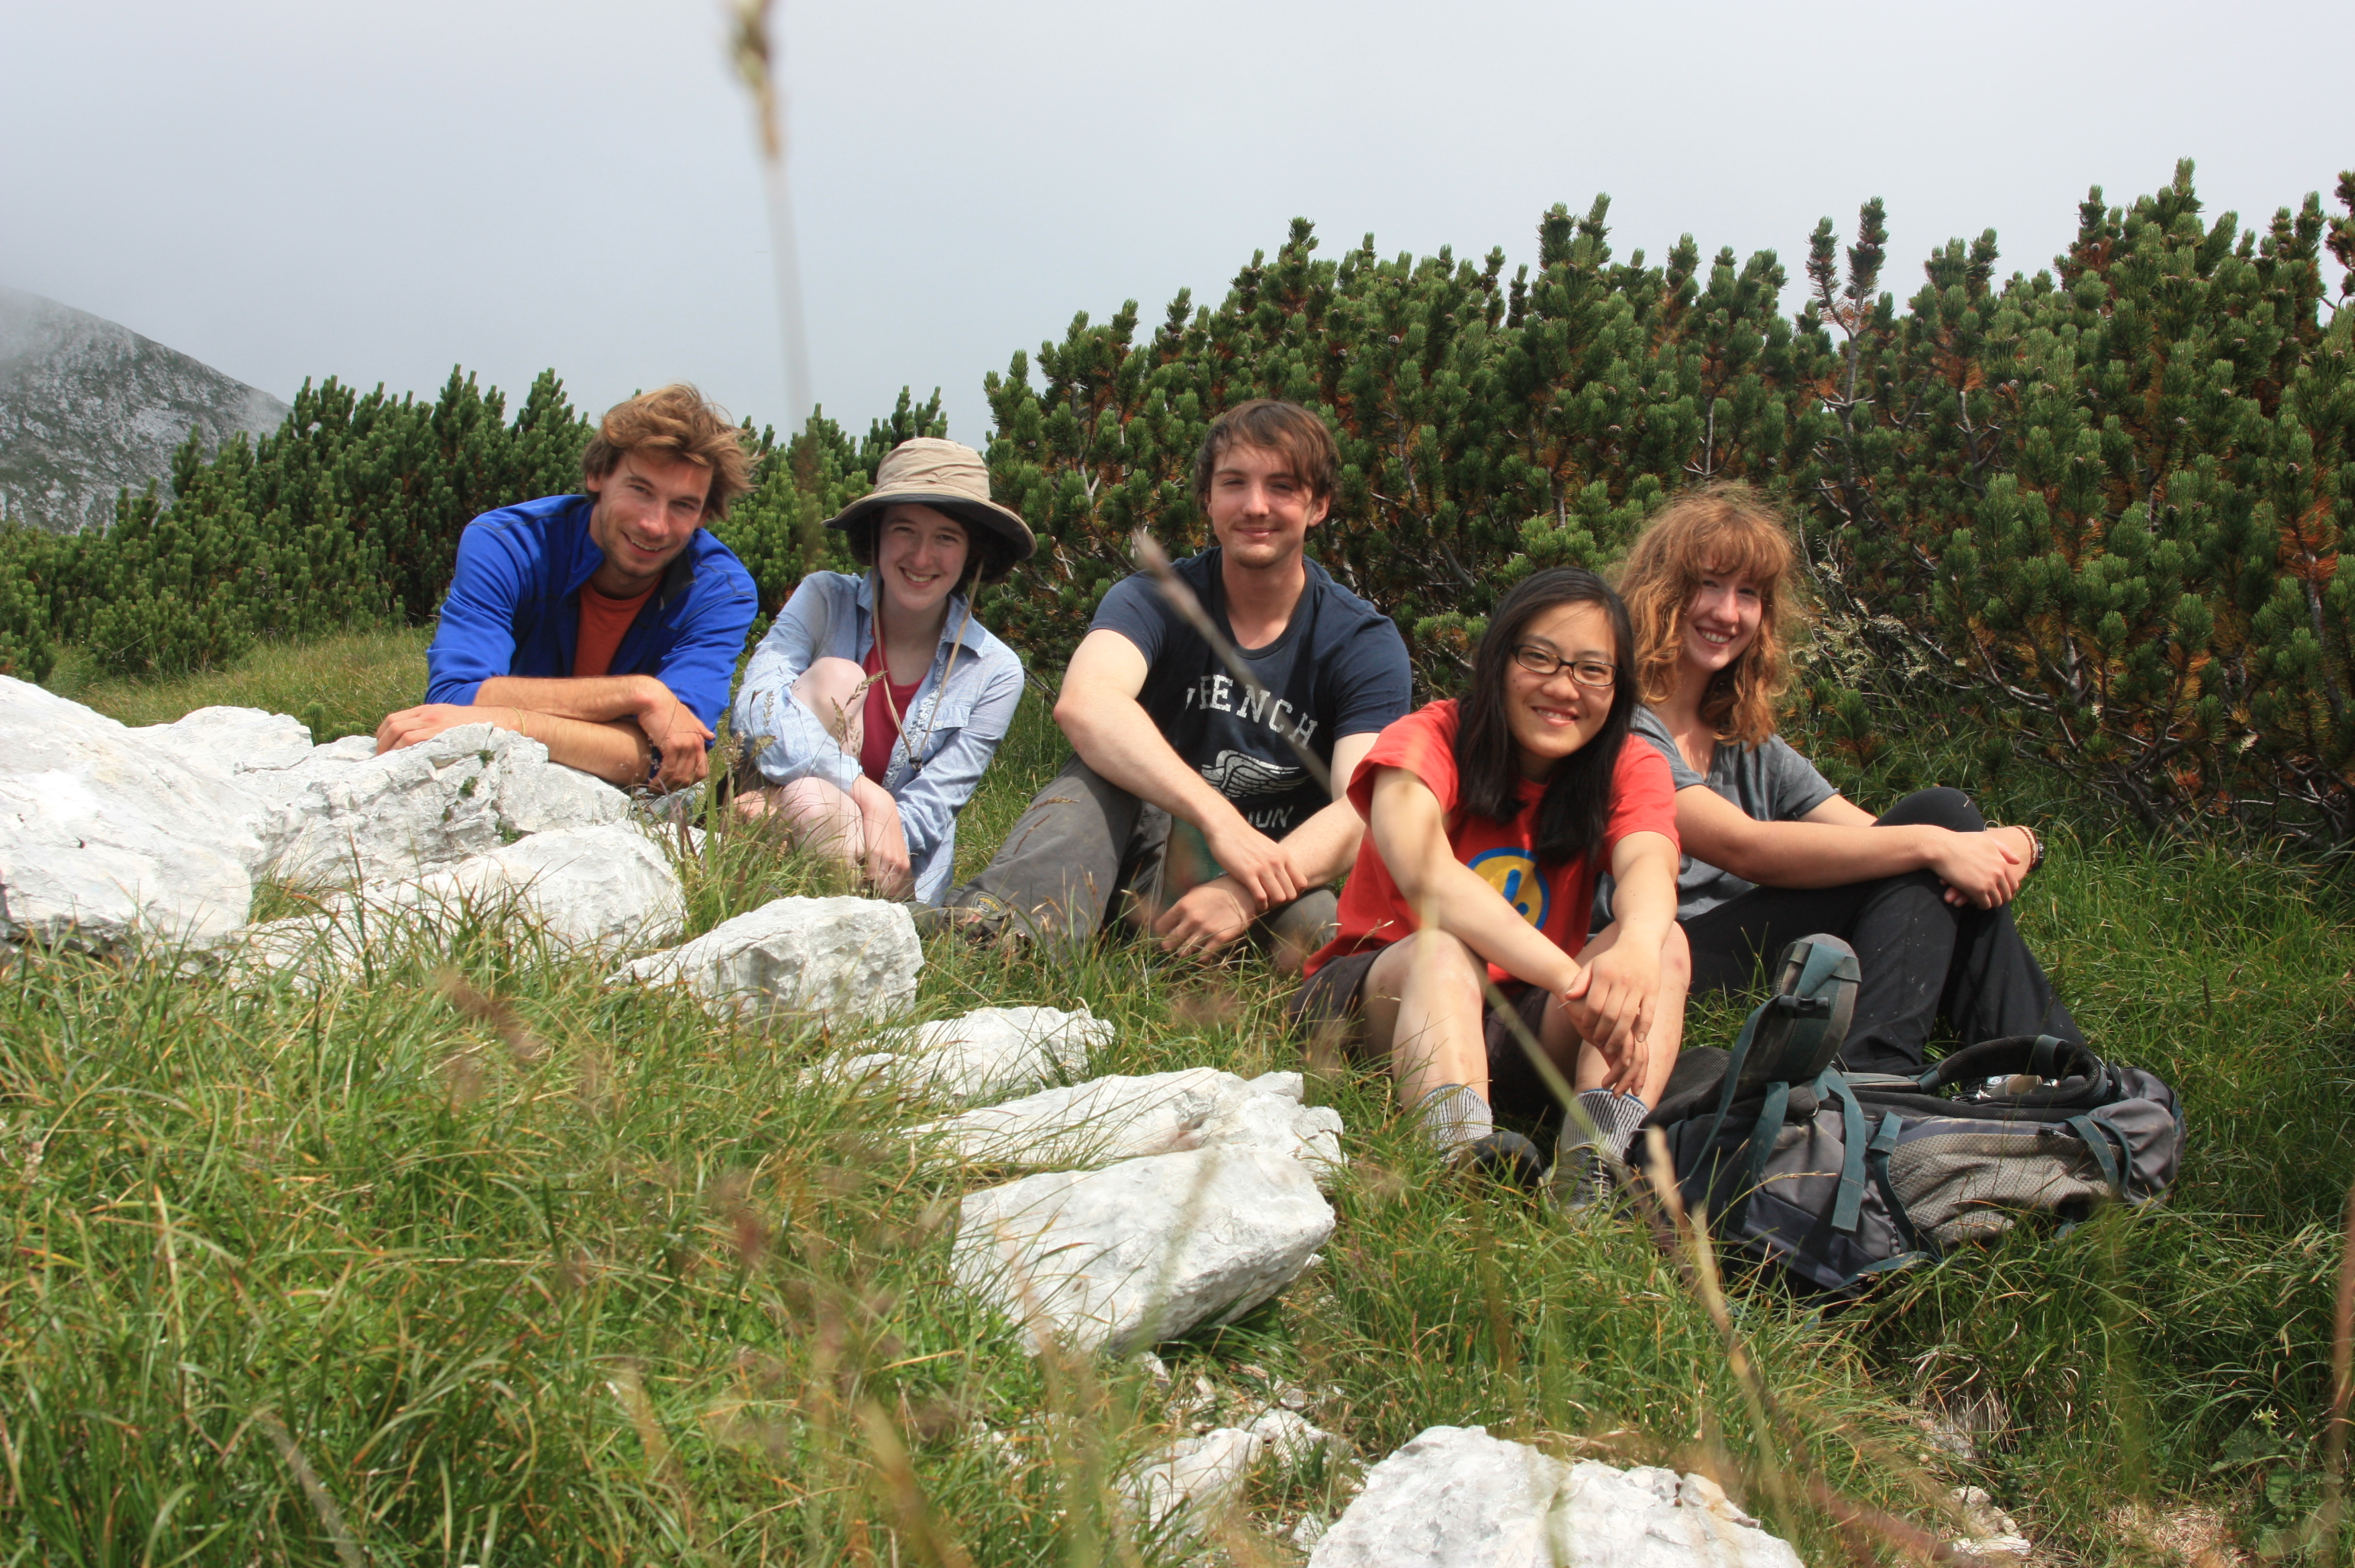
\includegraphics[width=\linewidth]{2011/alex_pitcher_award/2011-08-01-11.16.39-Gergely Ambrus-Canon450D-IMG_0769-Plateau--orig.jpg}}
            \caption{}\label{young gang 2011}
        \end{subfigure}
        \hfill
        \begin{subfigure}[t]{0.303\textwidth}
            \centering
            \frame{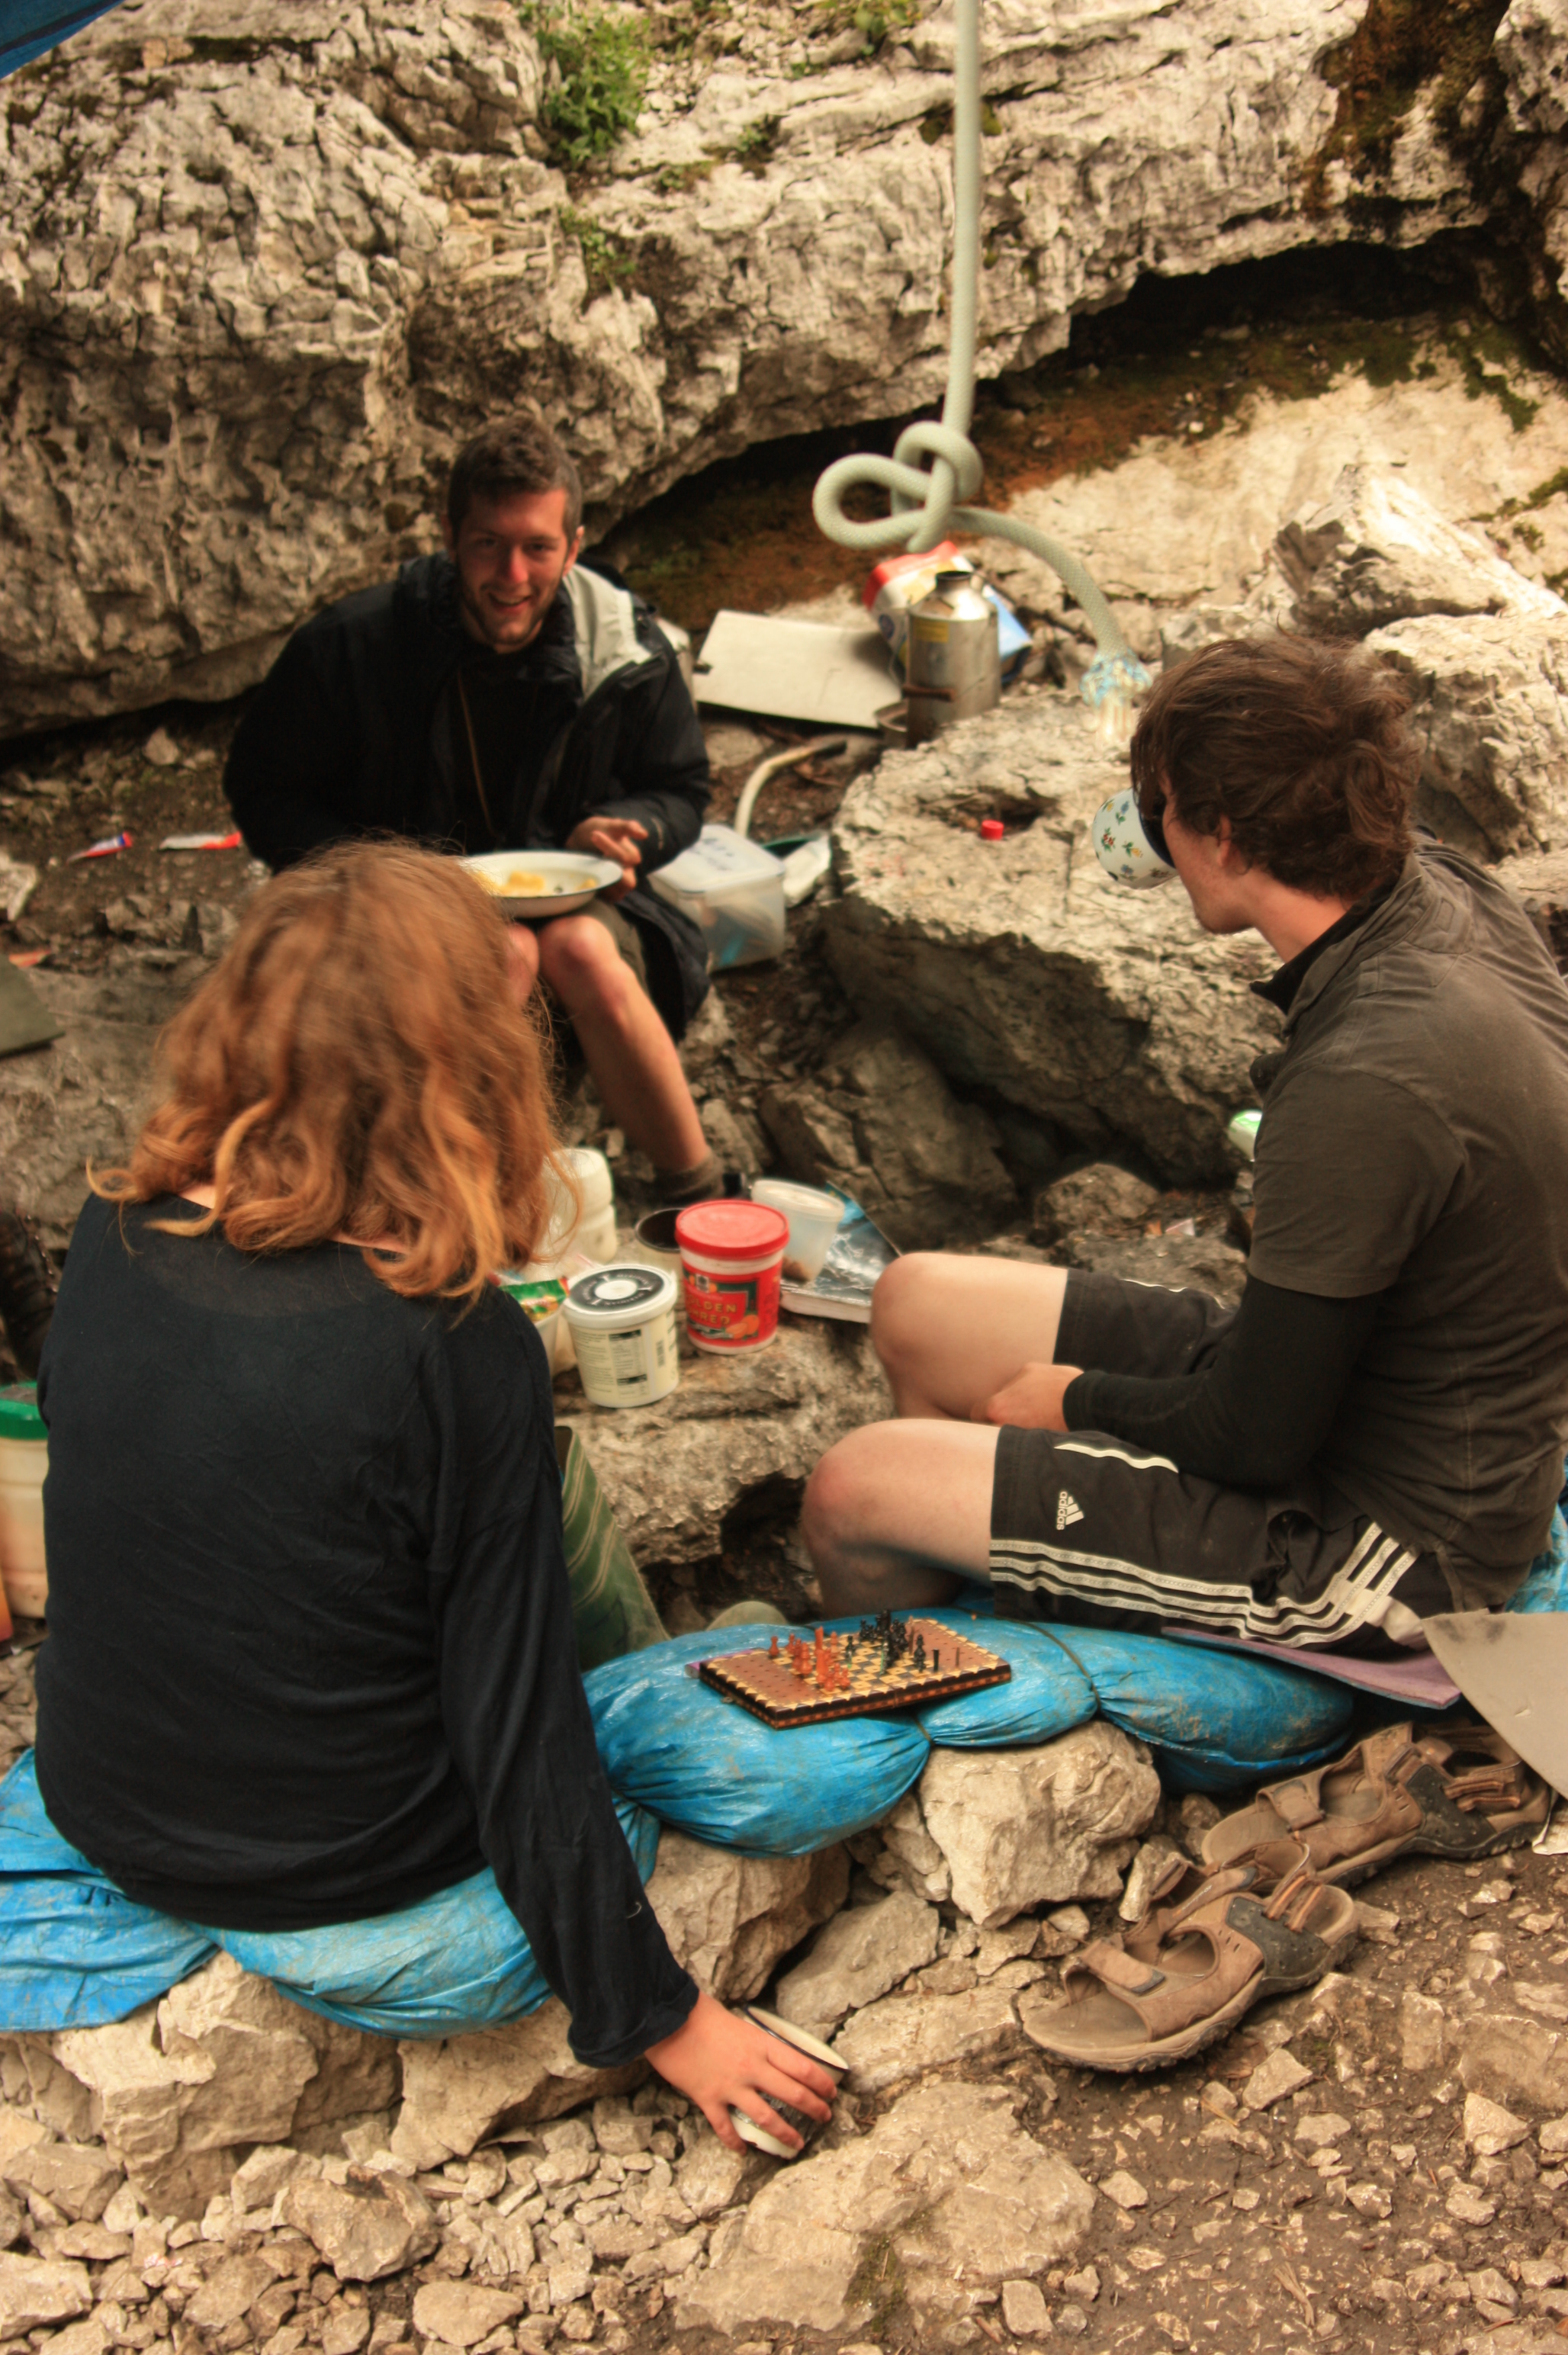
\includegraphics[width=\linewidth]{2011/alex_pitcher_award/2011-08-05-17.14.38-Gergely Ambrus-Canon450D-IMG_0929-Bivi--orig.jpg}}
            \caption{} \label{jonny dan kate}
        \end{subfigure}

        \vspace{0.3cm}
        
        \begin{subfigure}[t]{\textwidth}
            \centering
            \frame{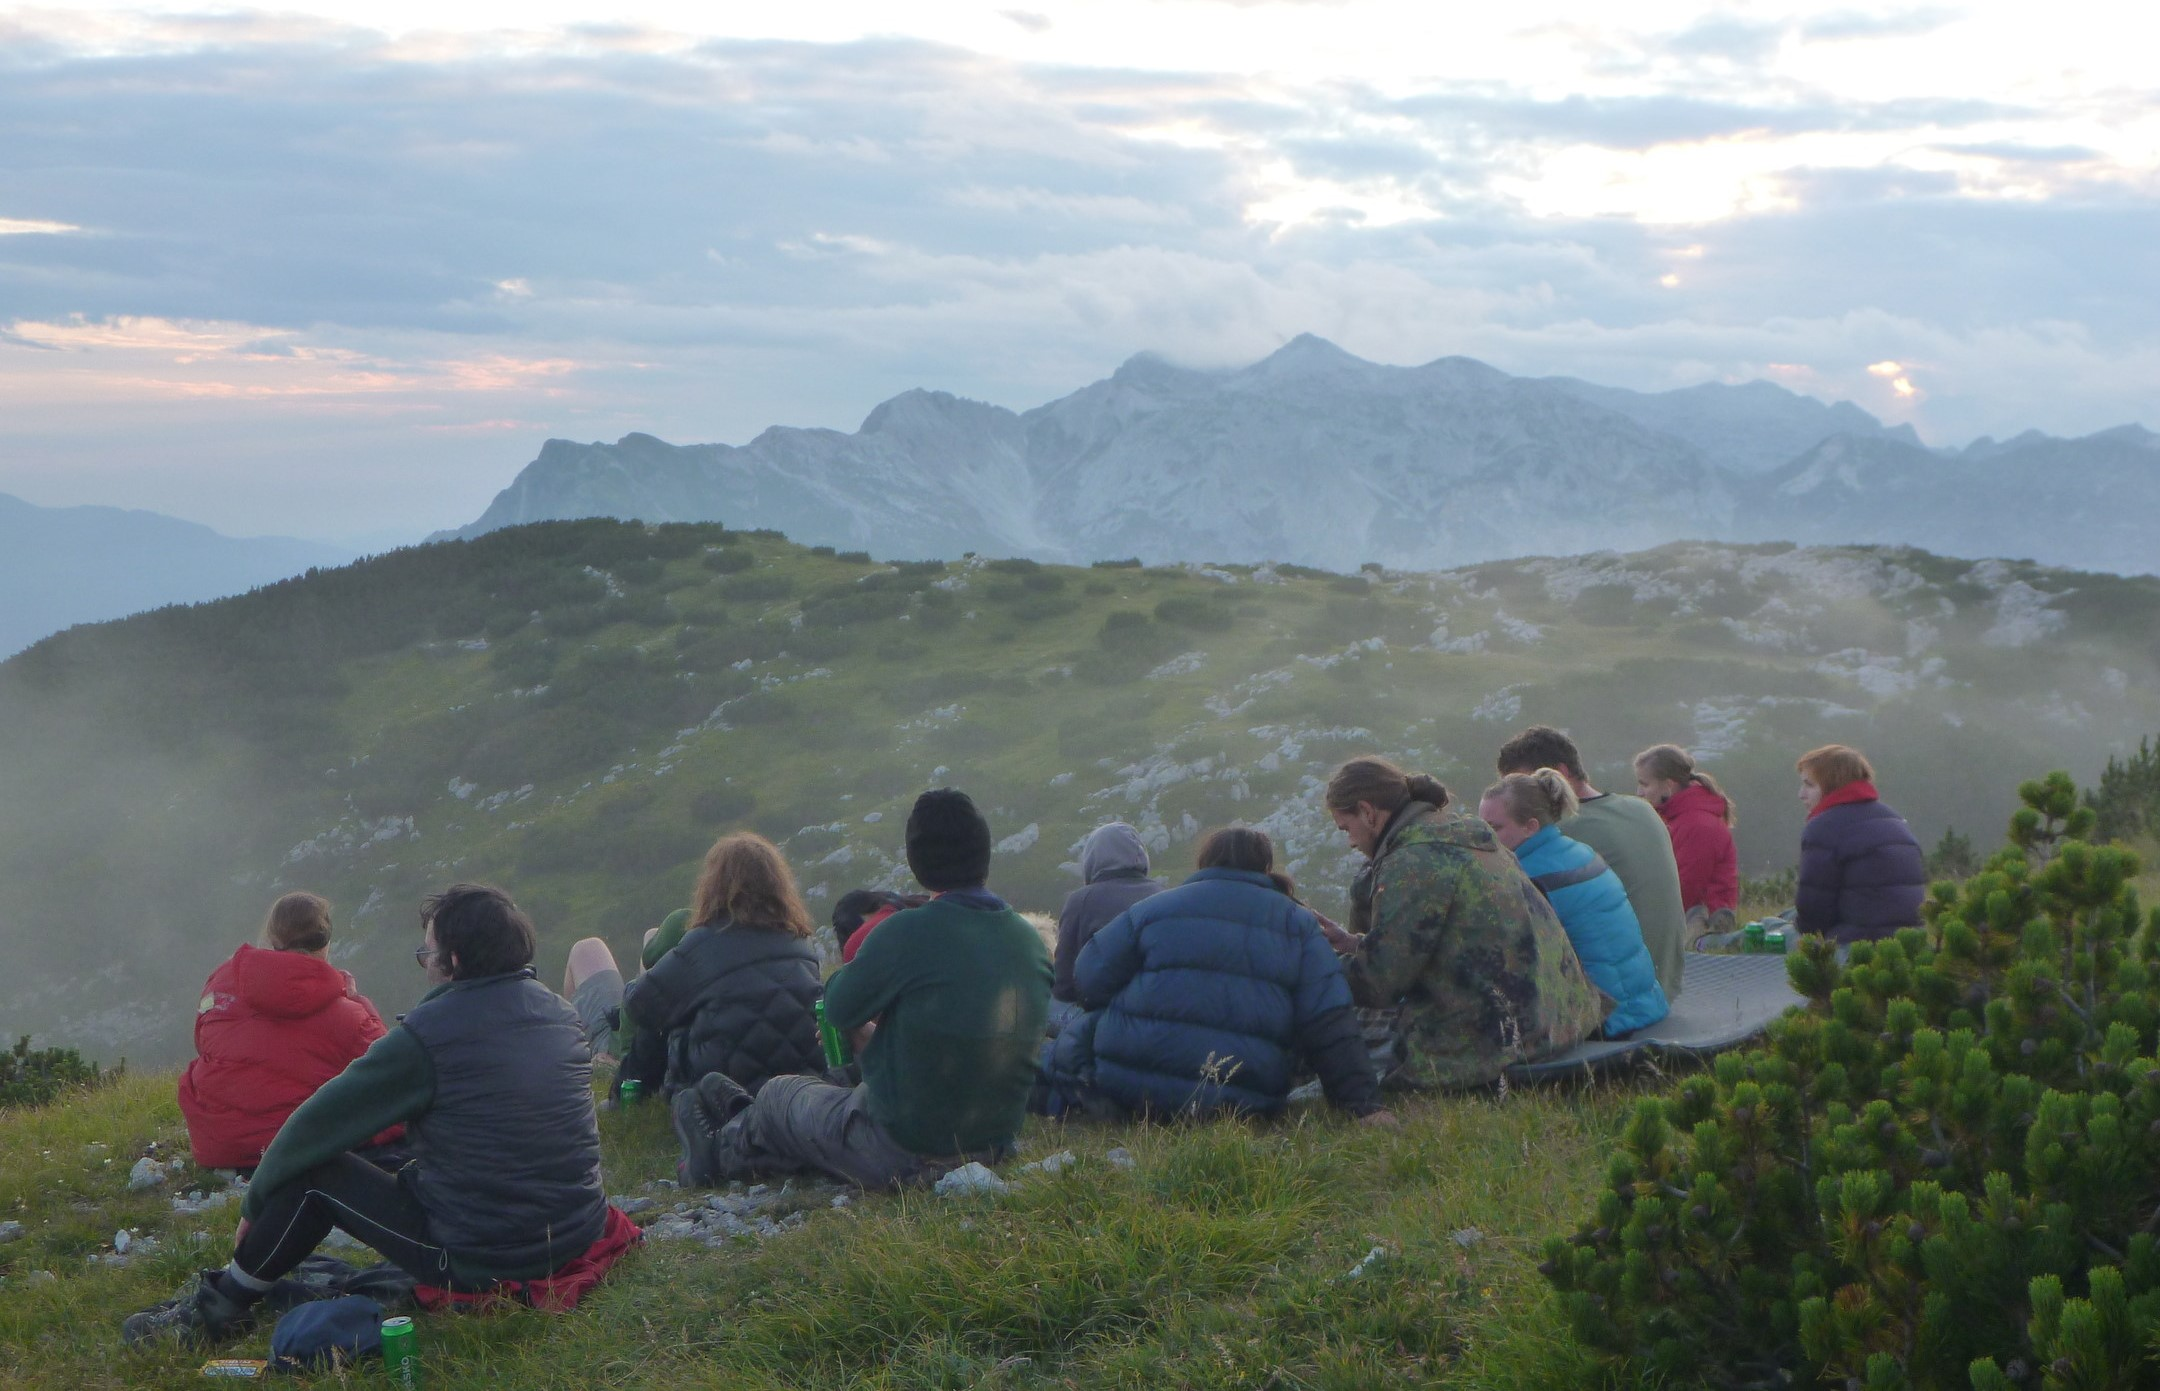
\includegraphics[width=\linewidth]{2011/alex_pitcher_award/2011-07-31-20.16.09-Grega-Panasonc DMC-FT2-071--orig.jpg}}
            \caption{} \label{cloudy sunset}
        \end{subfigure}
        
        \caption{Life up top. \textit{(a)} Gergely, Nia, Jonny, Clare and Kate.
            \textit{(b)} Hanging out in the bivi. \pic{Gergely Ambrus}
            \textit{(c)} Daily evening socialisation. \pic{Grega Maffi}
        }
    \end{figure*}

Here, I enjoyed an entirely different style of pushing to the style I
experience with Tetley. Not being experienced with a drill or with
putting bolts in myself, it was down to Dave to lead the pitch, this
required a tremendous amount of work from him and a large amount of
patience from me. 3 to 4 hours of shivering in the strong draft above
the pitch and the traverse had only extended about 10 metres
horizontally and about 5 metres vertically owing itself to the weakness
and unreliability of the rock. That, and it appeared that bolting on a
mud slope was tricky. Upon this futile first attempt we decided to head
to the bottom of \passage{Big Rock Candy Mountain} to assess our situation.

Before heading down on this trip I'd heard all manner of things about
\passage{Big Rock Candy Mountain}. To summarise, it wasn't seen to be one
of the nicer pitches in Slovenia and I'd been warned about a particular
free hanging rebelay. I descended tensely at first humming the tune to
\passage{Big Rock Candy Mountain} to calm myself. It didn't take long
before I started to enjoy the pitch and, aesthetically it remains my
favourite one in Slovenia. The mud slope soon changed into a vertical
pitch that descended into a large rift. Beyond this rift the whole
cavern opened up spectacularly before the rope left the wall at an
overhang and dropped into space. It was here that I came to face the
rebelay that I had been warned about.

Being free-hanging, it wouldn't
have been particularly enjoyable without any added complications,
especially with the drop below me. What made matters worse were the many
ropes that had been attached to the rebelay, seemingly going off in
different directions. Upon reattaching my descender, they helped to make
unclipping my cowstails slightly more difficult than on a normal
rebelay. It's at this point, the pace that I was humming \passage{Big Rock
Candy Mountain} at increased. Realised that I would have to use my hand
jammer to help release my short cowstail I attached it to the rope above
and removed the cowstail, feeling an immense relief. That is, until I
noticed that all my weight was now on my hand jammer. Standing up in the
length of rope above me I finally freed myself and began to descend down
the remaining length of the pitch, quite shaken.

\margininbox{4.8.2011 9:50am}{

Despite not discovering much yesterday, it's
been a great trip, especially experiencing some expedition bolting
(cold) and de-rigging (fun). Hopefully I'll be back in the next week,
even if it is for a de-rig. No sign of Izi + Gergely on the night train
-- hopefully they've found something exciting at \passage{Stuck in
Paradise}.\name{Jonny}}{\logbook}

It was from here we
noticed that our initial attempt had been futile. The small hole that
Dave had noticed previously turned out to be what looked like a separate
chamber of comparable size to \passage{BRCM}. Unfortunately, climbing over to it
would have to wait for another team.

\begin{pagefigure}
\checkoddpage \ifoddpage \forcerectofloat \else \forceversofloat \fi
   \centering
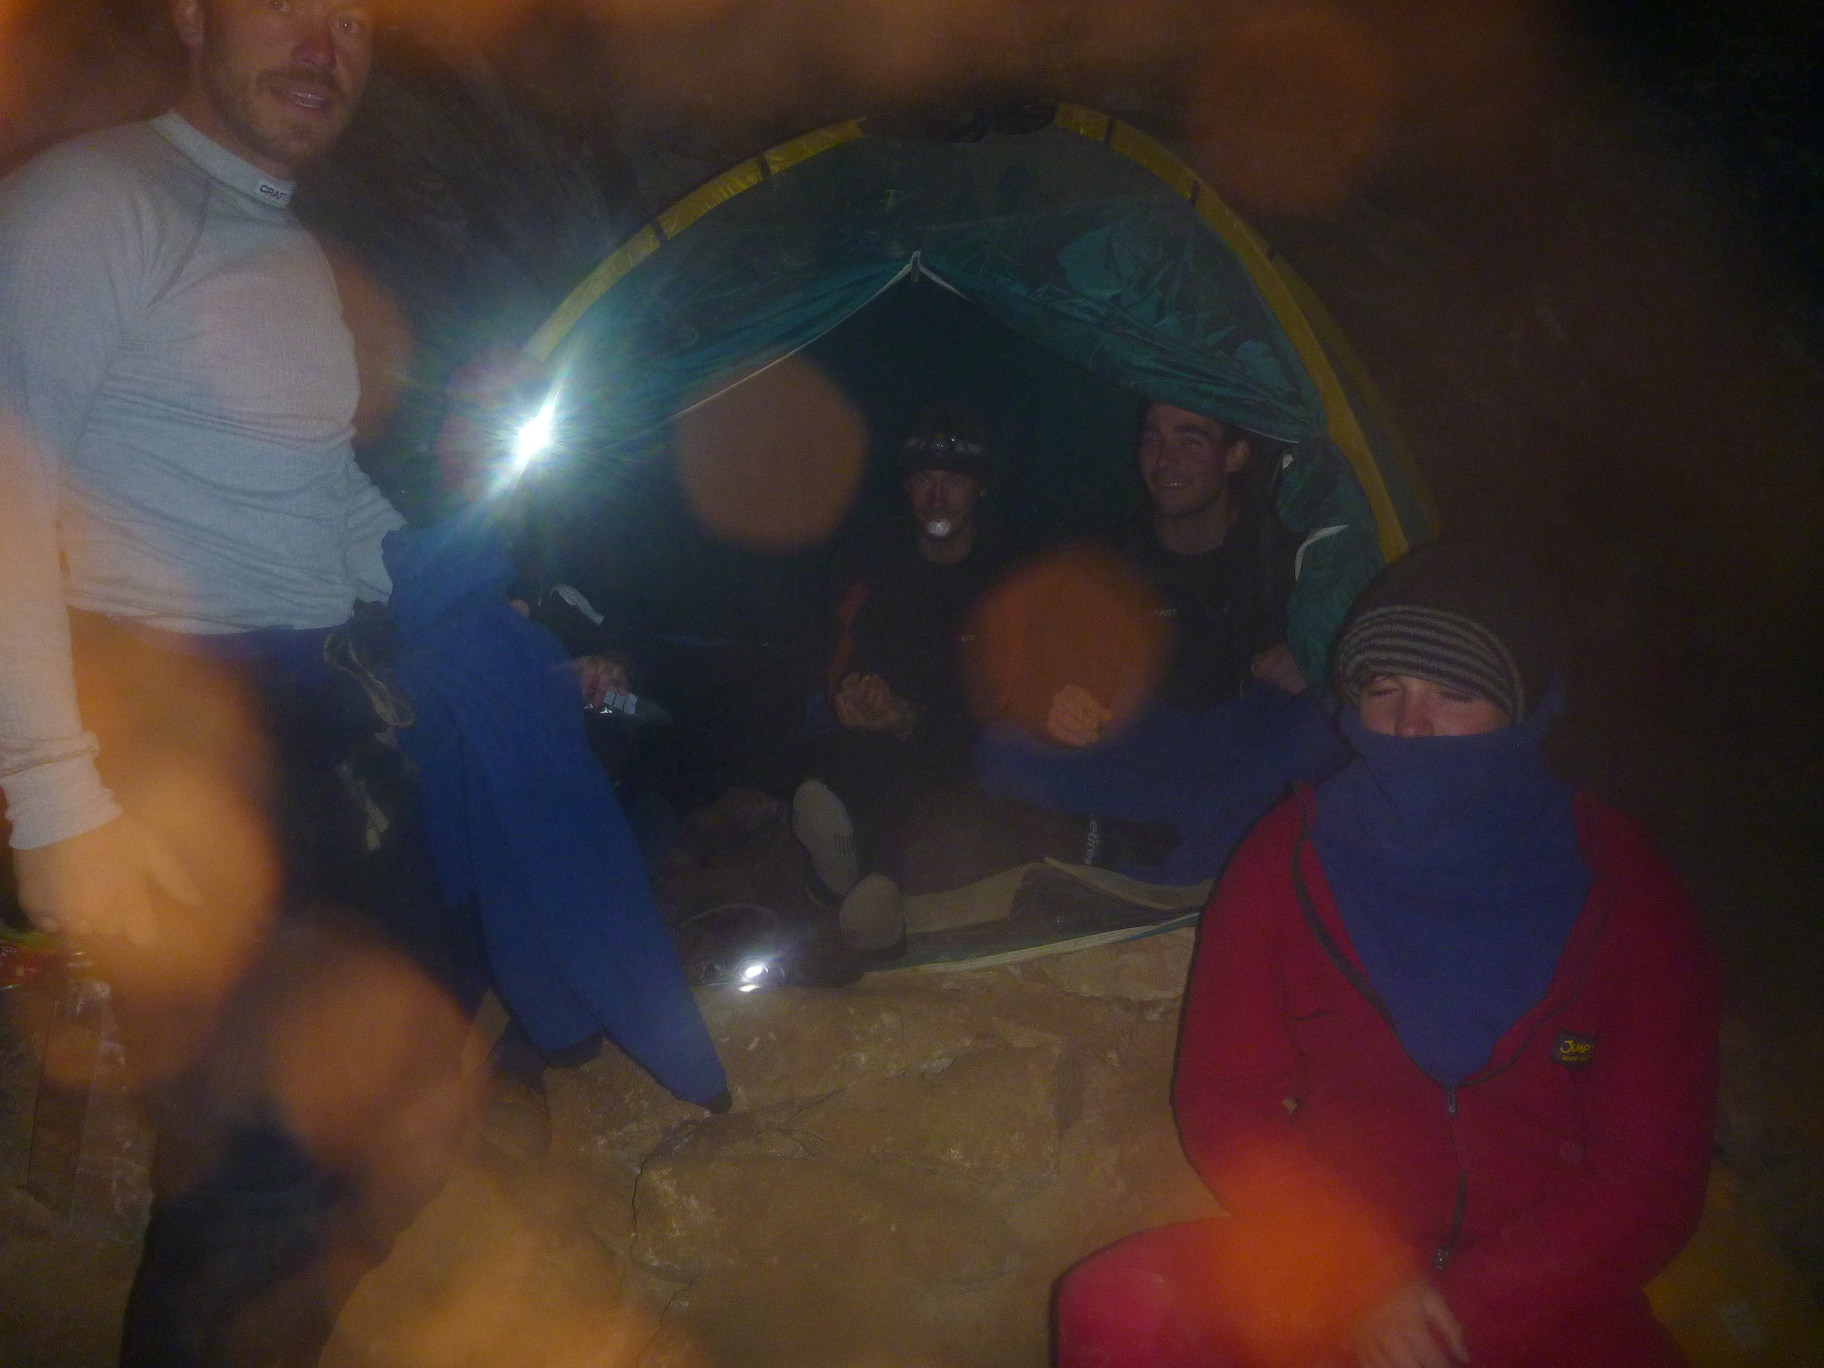
\includegraphics[width = \textwidth]{2011/alex_pitcher_award/2011-08-03-09.45.02-Grega-Panasonc DMC-FT2-104-camp x-ray--orig.jpg}
\caption{Maffi, Jonny and others below ground at camp \passage{X-Ray}. \pic{Grega Maffi}} \label{jonny x-ray}
\end{pagefigure}

Feeling defeated we returned to
\passage{Friendship Gallery} and had a look at on of the other leads that
had been discovered out of curiosity. Unfortunately, we were unable to
push any further cave. We rested, discussed our findings with other
cavers and exited the cave the next day, this time taking a tackle bag.
Whilst carrying the equipment out made sections such as \passage{Pink} and
the \passage{Urinal series} more awkward, it helped to increase my confidence
within the cave.



